\section{Grundlegende Architektur des Modells}
\label{sec:aufbauModel}

\begin{wrapfigure}{r}{0.5\columnwidth}
    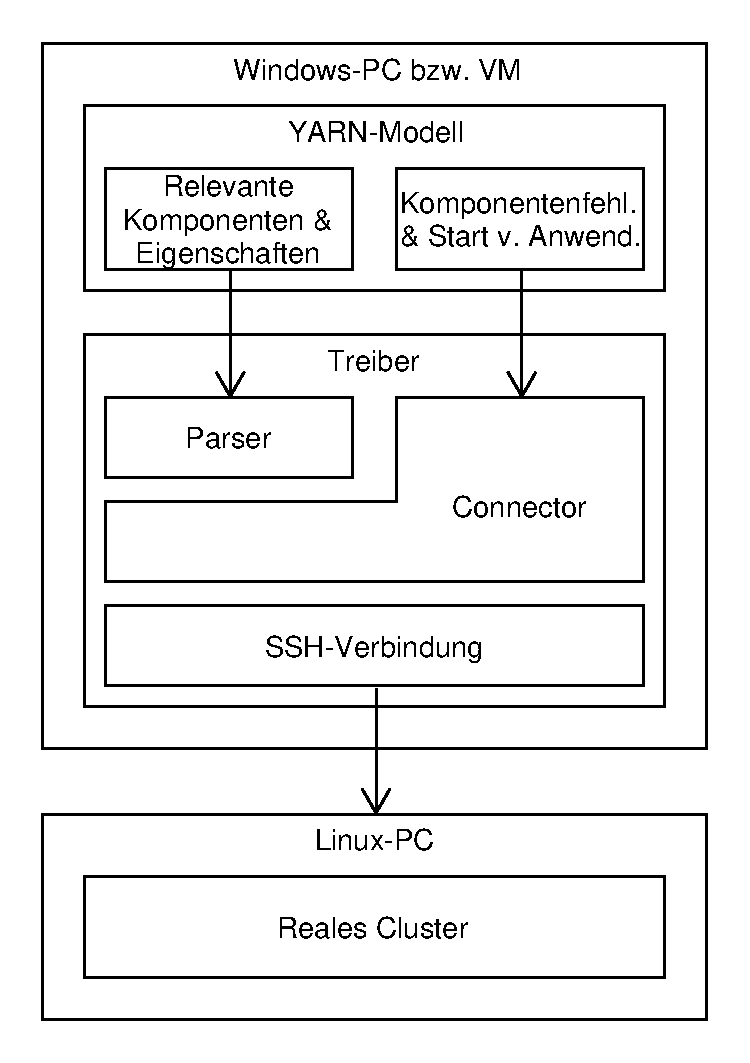
\includegraphics[width=0.5\columnwidth]
    {./images/modelArchitecture.pdf}
    \caption{Grundlegende Architektur des Gesamtmodells}
    \label{fig:modelArchitecture}
\end{wrapfigure}

Um Hadoop mit der Selfbalancing"=Komponente mit den in \autoref{sec:predictions} beschriebenen Behauptungen prüfen zu können, wird mithilfe des \ac{ss}"=Frameworks ein vereinfachtes Modell entwickelt.

Die rechts abgebildete \autoref{fig:modelArchitecture} beschreibt die grundlegende Architektur des Modells für diese Fallstudie.
Die Fallstudie besteht aus den drei Schichten des YARN"=Modells selbst, dem Treiber zum Herstellen der Verbindung zwischen dem Modell und dem realen Cluster sowie dem realen Cluster selbst.

Das eigentliche YARN"=Modell bildet die grundlegende Architektur von YARN bzw. YARN"=Anwendungen stark vereinfacht ab.
Es enthält daher nur die für diese Fallstudie relevanten Komponenten und Eigenschaften sowie die Definitionen der Komponentenfehler.

Die Verbindung zwischen dem Modell und dem realem Cluster bildet der Treiber als eigenständige Schicht.
Der Treiber besteht aus folgenden Komponenten:

\begin{description}
    \item [Parser] \hfill \\
        Verarbeitet die Monitoring"=Ausgaben vom realen Cluster und konvertiert diese für die Nutzung im YARN"=Modell.
    \item [Connector] \hfill \\
        Abstrahiert die Verbindung zum realen Cluster und die dabei auszuführenden Befehle.
    \item [SSH"=Verbindung]  \hfill \\
        Stellt die Verbindung zum realen Cluster her.
\end{description}

Der Zugriff mithilfe des Treibers auf das reale Cluster im Rahmen des Monitoring wird mithilfe des Parsers durchgeführt, welcher wiederum den Connector nutzt.
Bei anderen Zugriffen wie \zB die Injizierung und das Reparieren von Komponentenfehlern oder dem Starten von Anwendungen wird vom YARN"=Modell mithilfe des Connectors auf das reale Cluster zugegriffen.

Die Umsetzung des realen Clusters wird im folgenden \autoref{sec:aufbauCluster} beschrieben.
Die Umsetzung des YARN"=Modells und des Treibers wird im folgenden \autoref{chap:modell} beschrieben.
